
\section{Implementation}
\label{sec:imp}

\subsection{MADlib}

TODO: explains how MADlib works. What's the point of it, what it does?

\subsection{Genetic Programming for symbolic regression}
\subsubsection{Background}

Genetic programming is a subset of evolutionary algorithms, which is a family of optimization algorithms based on the principle of \textbf{Darwinian natural selection}. As part of natural selection, a given environment has a population of individuals that compete for survival and reproduction. The ability of each individual to achieve these goals determines their chance to have children, in other words to pass on their genes to the next generation of individuals, who for genetic reasons will have an increased chance of doing well, even better, in realizing these two objectives.

~~\\
This principle of continuous improvement over the generations is taken by evolutionary algorithms to optimize solutions to a problem. In the \textbf {initial generation}, a \textbf{population} composed of different \textbf {individuals} is generated randomly or by other methods. An individual is a solution to the problem, more or less good: the quality of the individual in regards to the problem is called \textbf{fitness}, which reflects the adequacy of the solution to the problem to be solved. The higher the fitness of an individual, the higher it is likely to pass some or all of its genotype to the individuals of the next generation.

~~\\
An individual is coded as a \textbf{genotype}, which can have any shape, such as a string (genetic algorithms), a vector of real (evolution strategies) or in our case a tree (genetic programming). Each genotype is transformed into a \textbf{phenotype} when assessing the individual, i.e. when its fitness is calculated. In some cases, the phenotype is identical to the genotype: it is called \textbf{direct coding}. Otherwise, the coding is called indirect. For example, suppose you want to optimize the size of a rectangular parallelepiped defined by its length, height and width. To simplify the example, assume that these three quantities are integers between 0 and 15. We can then describe each of them using a 4-bit binary number. An example of a potential solution may be to genotype 0001 0111 01010. The corresponding phenotype is a parallelepiped of length 1, height 7 and width 10.

~~\\
During the transition from the old to the new generation are called \textbf{variation operators}, whose purpose is to manipulate individuals. There are two distinct types of variation operators:
\begin{itemize}
	\item the \textbf{mutation operators}, which are used to introduce variations within the same individual, as genetic mutations;
	\item the \textbf{crossover operators}, which are used to cross at least two different genotypes, as genetic crosses from breeding.
\end{itemize}

The figure \ref{fig:algorithmes_evolutionnistes_synopsis} summarizes how an evolutionary algorithm works.

\begin{figure}[htb]
	\centering
		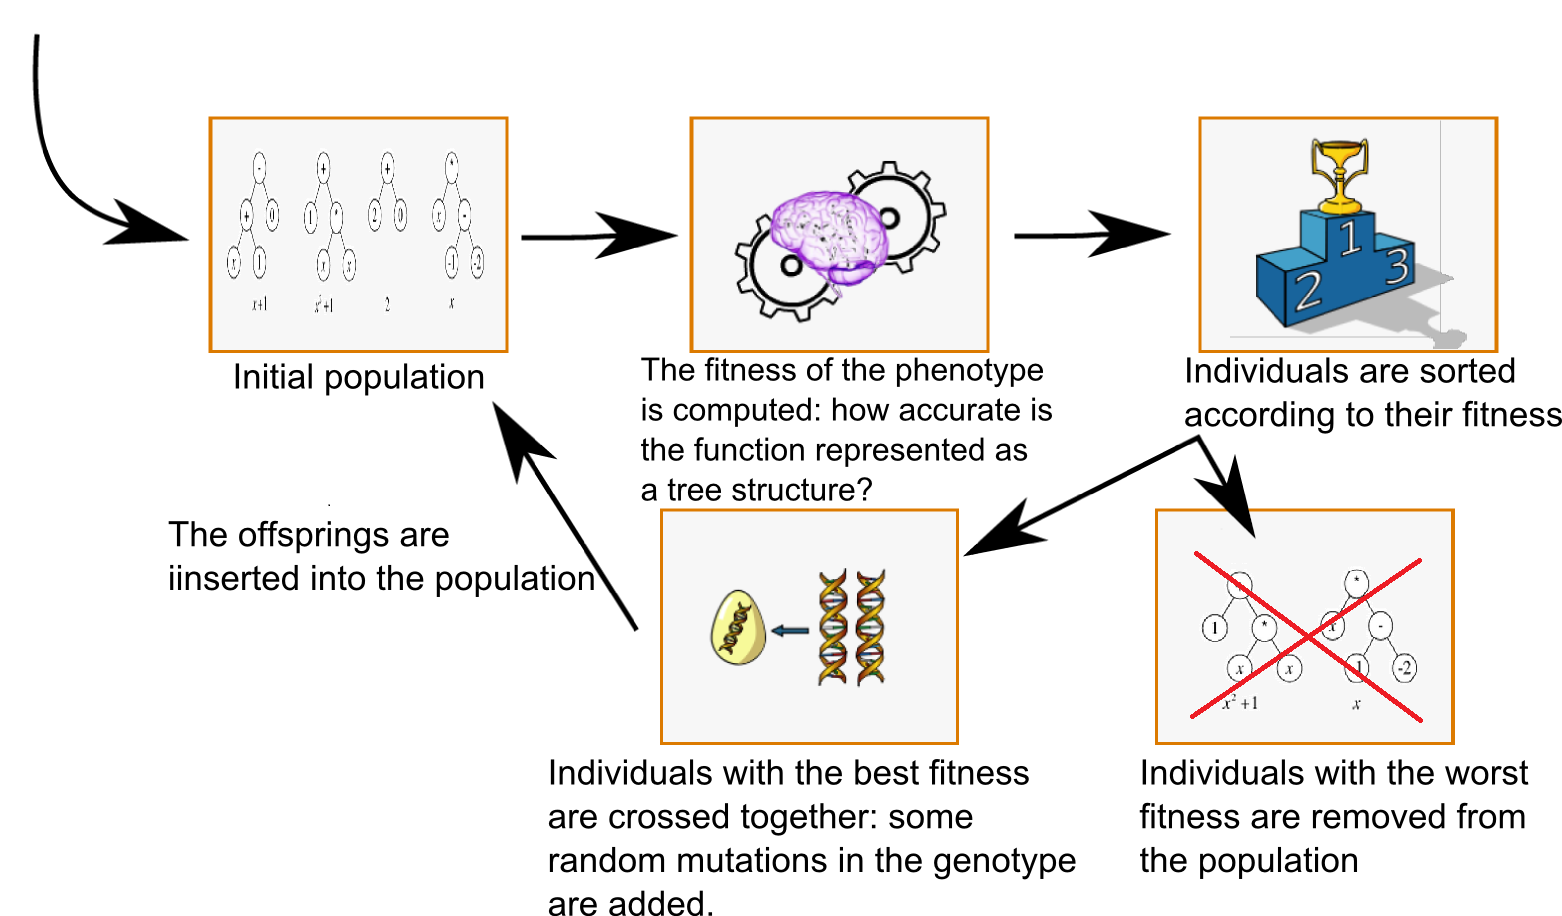
\includegraphics[width=0.8\textwidth]{genetic_programming_regression_synopsis.png}
	\caption[Functioning of an evolutionary algorithm]{Functioning of an evolutionary algorithm: from an initial population of solutions (in symbolic regression, a solution is the tree representing a fraction), they are ranked according to their fitness, the worst ones are eliminated and the best ones are used to produce new solutions.}
	\label{fig:algorithmes_evolutionnistes_synopsis}
\end{figure}

\begin{figure}[htb]
	\centering	
		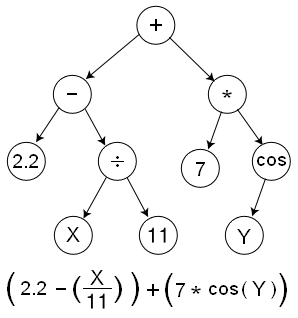
\includegraphics[scale=0.45]{Genetic_Program_Tree.png}
	\caption[A function represented as a tree structure.]{A function represented as a tree structure. Source: Wikipedia}
	\label{fig:Genetic_Program_Tree}
\end{figure}

~~\\
Genetic programming is a perfect suit for symbolic regression. The term "symbolic regression" represents the process during which measured data are fitted by suitable mathematical formula like $x^2 + C$, $sin(x) + 1/e^x$,  etc. The figure \ref{fig:Genetic_Program_Tree} shows how a formula can the represented as a tree. This process is quite well known amongst mathematician and is used when some data of unknown process are obtained. The domain of symbolic regression is of functional nature, i.e. it consists of a function set like ($sin()$, $cos()$, $gamma()$, $MyFunction()$,...) and so called terminal set ($t$, $x$, $p$, ...). The final program is synthesized from a mixture of both sets, and can be quite complicated from a structural point of view. We plan to use genetic programming for symbolic regression in order to unravel unknown relation between some given attributes of a relation. 


\subsubsection{Madlib Implementation}
TODO

DEAP

Appendix \ref{sec:app:implementation} gives details on the technical aspects of the implementation.

\subsection{Adaptive Boosting}
\subsubsection{Background}
Boosting is one of the most important developments in classification methodology. Boosting works by iteratively applying a classification algorithm to re-weighted versions of the training data and then taking a weighted majority vote of the sequence of classifiers thus produced. For many classification algorithms, this simple strategy results in dramatic improvements in performance. While boosting has evolved over the years, we focus on the most commonly used version of boosting known as Adaptive Boosting (AdaBoost) for binary classification developed by Freund and Schapire~\cite{boost96}.

Let us look at a concise description of AdaBoost in a two-class classification setting. We have training data $(x_1, y_1), \ldots, (x_n, y_n)$ with $x_i$ a vector valued feature and $y_i = -1\text{ or }1$. We define $F(x) = \sum_1^M{c_mf_m(x)}$ where each $f_m(x)$ is a classifier producing values $1\text{ or }-1$ and $c_m$ are constants; the corresponding prediction is $\text{sign}(F(x))$. The AdaBoost procedure trains the classifiers $f_m(x)$ on weighted versions of the training sample, giving higher weight to cases that are currently misclassified. This is done for a sequence of weighted samples, and then the final classifier is a linear combination of the classifiers from each stage. The pseudocode for AdaBoost is given in Figure~\ref{fig:adaproc}.

\begin{figure}[ht]
\centering
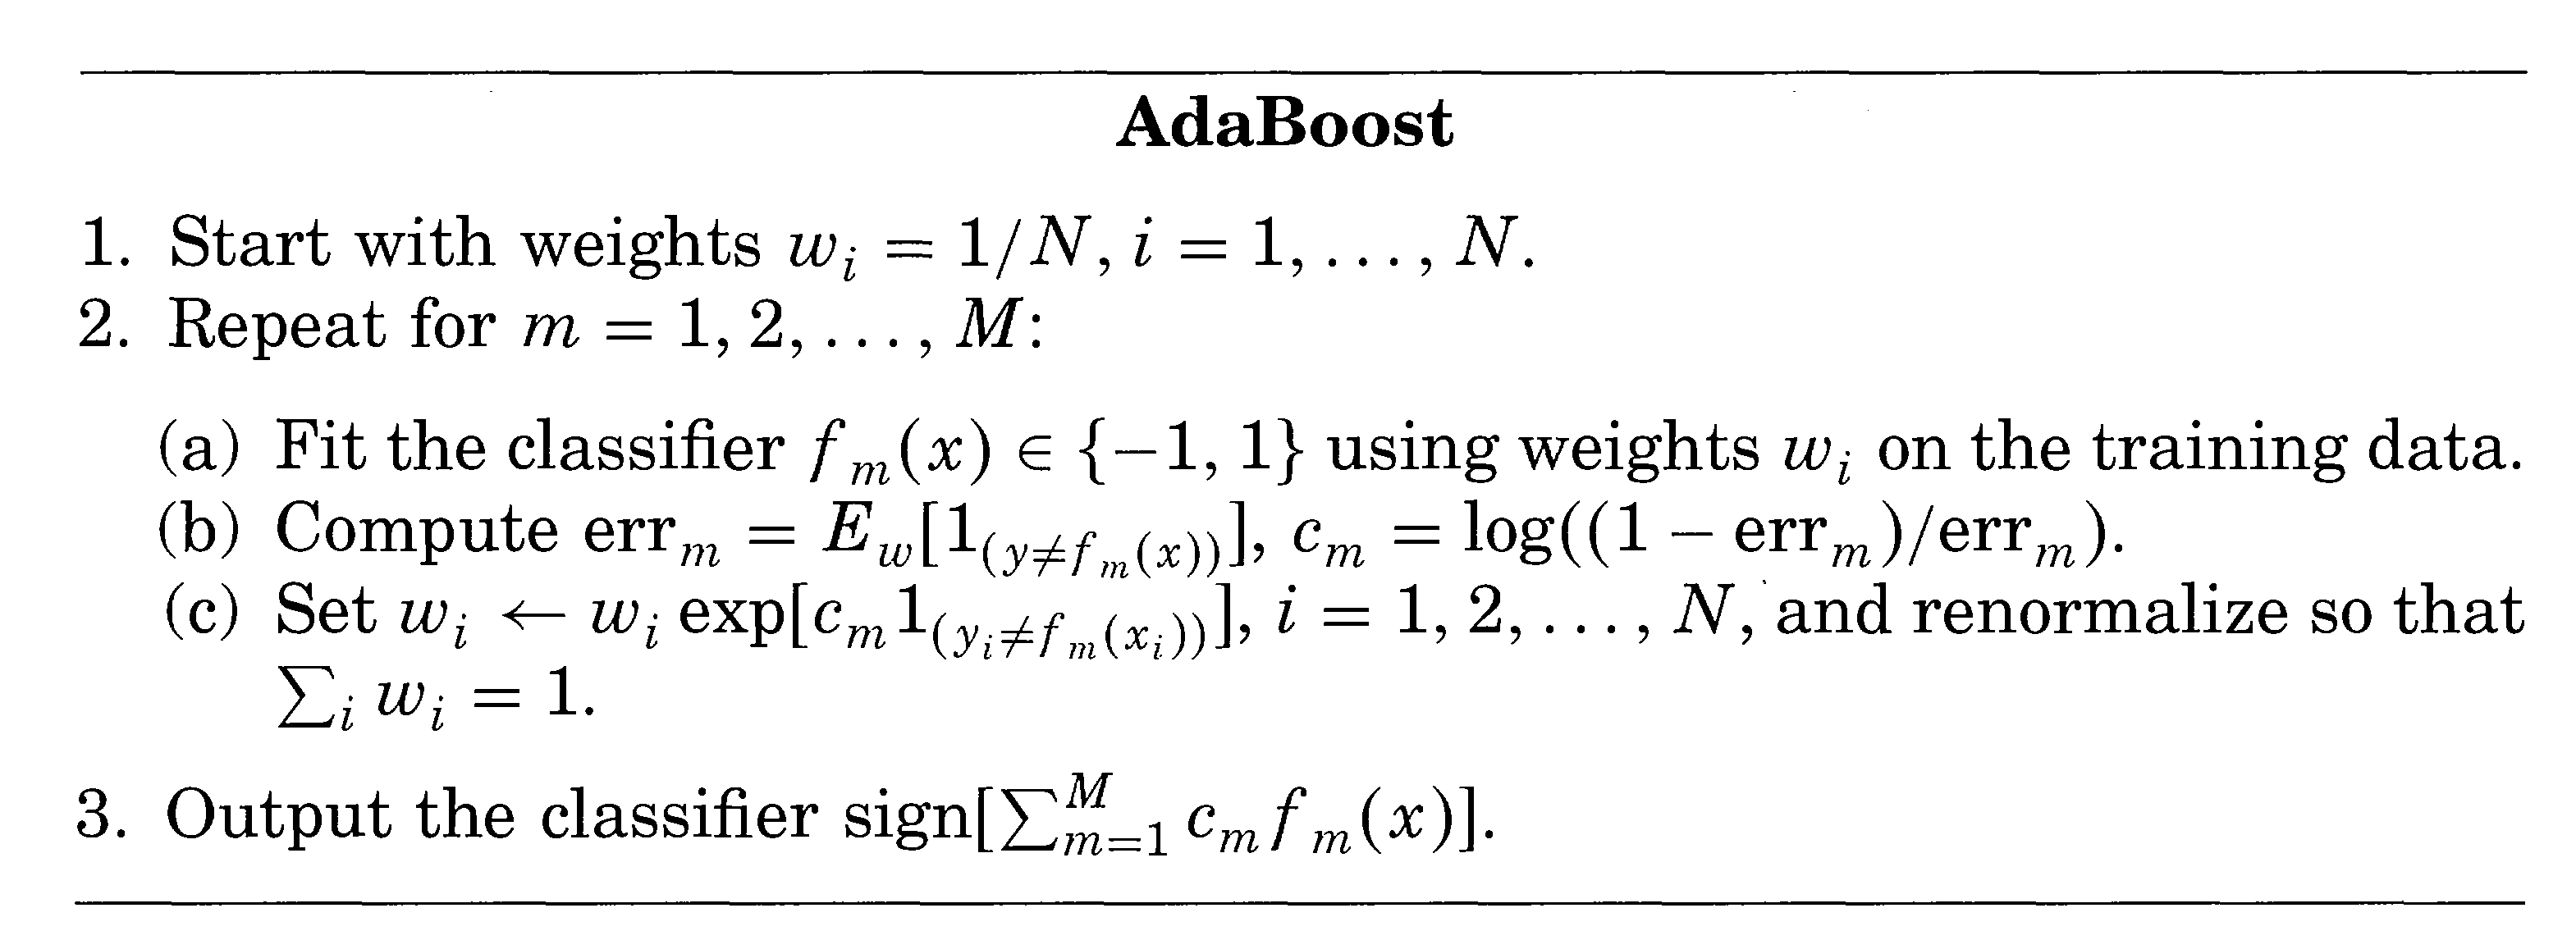
\includegraphics[width=0.8\textwidth]{ada.png}
\caption{AdaBoost algorithm. $E_w$ represents expectation over the training data with weights $w=(w_1,w_2,\ldots,w_N)$ and $I_{(S)}$ is the indicator of the set $S$~\cite{alr00}.}
\label{fig:adaproc}
\end{figure}

We used ``Stumps'' as weak learners. Stumps are single-split trees with only two terminal nodes. Stumps are simple to implement, typically have low variance and success of boosting depends on variance reduction~\cite{alr00}.


\subsubsection{Madlib Implementation}
